\section{Energy Consumption in CPUs}

Two sources of energy consumption in a CPU can be distinguished; static and
dynamic. Static energy consumption is caused by a small current continously
leaking through the transistors, while dynamic is due to charges being moved
towards ground when transistors are toggling \cite{wolf}.
\autoref{fig:staticdynamic} shows how current flows through a NOT gate at the
transistor level. The green arrow indicates where static leakage occurs and the
two red arrows shows where charges escapes when switching. As feature size
decreases, a significant part of overall energy consumption is due to static
leakage \cite{nguyen2003minimization}. This means that simply powering the chip
without any toggling generates a significant amount of heat
\cite{kim2003leakage,martin2002combined}. While static power consumption origins
from transistor size and layout, dynamic power consumption can be treated at the
architectural level by minimizing transistor switching.

\begin{figure}[tbh]
    \centering
    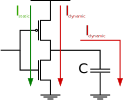
\includegraphics[width=0.4\textwidth]{figs/static-dynamic.pdf}
    \caption{Static and dynamic power through a PMOS and NMOS transistor.}
    \label{fig:staticdynamic}
\end{figure}
